\documentclass[aspectratio=169, 10pt]{beamer}

% ============================================================================
% THEME: Metropolis + custom deep teal / coral palette
% ============================================================================
\usetheme[progressbar=frametitle, numbering=fraction, block=fill]{metropolis}

\definecolor{primaryDark}{HTML}{1B2A41}
\definecolor{primaryTeal}{HTML}{00838F}
\definecolor{accentCoral}{HTML}{E85D75}
\definecolor{accentGold}{HTML}{F4A261}
\definecolor{successGreen}{HTML}{2A9D8F}

\setbeamercolor{frametitle}{bg=primaryDark, fg=white}
\setbeamercolor{progress bar}{fg=accentCoral, bg=primaryDark!20}
\setbeamercolor{title separator}{fg=accentCoral}
\setbeamercolor{alerted text}{fg=accentCoral}
\setbeamercolor{example text}{fg=successGreen}
\setbeamercolor{block title}{bg=primaryTeal, fg=white}
\setbeamercolor{block body}{bg=primaryTeal!8, fg=black}
\setbeamercolor{block title alerted}{bg=accentCoral, fg=white}
\setbeamercolor{block body alerted}{bg=accentCoral!8, fg=black}
\setbeamercolor{block title example}{bg=successGreen, fg=white}
\setbeamercolor{block body example}{bg=successGreen!8, fg=black}

\usepackage{amsmath, amssymb, amsfonts, amsthm}
\usepackage{graphicx}
\usepackage{tikz}
\usetikzlibrary{shapes, arrows.meta, positioning}

\newcommand{\R}{\mathbb{R}}
\newcommand{\E}{\mathbb{E}}
\newcommand{\Prob}{\mathbb{P}}
\DeclareMathOperator{\Var}{Var}
\DeclareMathOperator{\Cov}{Cov}
\DeclareMathOperator{\sgn}{sign}
\DeclareMathOperator*{\argmin}{arg\,min}
\newcommand{\Ind}[1]{\mathbb{I}\{#1\}}
\newcommand{\cX}{\mathcal{X}}
\newcommand{\cY}{\mathcal{Y}}
\newcommand{\cS}{\mathcal{S}}
\newcommand{\cR}{\mathcal{R}}

\title{The Case for Voluntary Disclosure}
\subtitle{Strategic Feature Revelation in Regression and Classification}
\author{Author 1 \and Author 2}
\date{2026}

\begin{document}

% ======================= SLIDE 1: TITLE =======================
{
\setbeamercolor{background canvas}{bg=primaryDark}
\begin{frame}[plain, noframenumbering]
  \vfill
  \begin{center}
    {\Huge\color{white}\textbf{The Case for Voluntary Disclosure}}\\[12pt]
    {\Large\color{accentCoral}Strategic Feature Revelation in Regression \& Classification}\\[20pt]
    {\color{white!70}Author 1\textsuperscript{1} \quad \& \quad Author 2\textsuperscript{2}}\\[6pt]
    {\small\color{accentGold}Strategic Learning with Heterogeneous Preferences}
  \end{center}
  \vfill
\end{frame}
}

% ======================= SLIDE 2: MOTIVATION =======================
\begin{frame}{Motivation \& Core Question}
  \begin{columns}[T]
    \begin{column}{0.55\textwidth}
      \textbf{Setting:} A predictive model relies on features from strategic participants.
      \vspace{4pt}
      \begin{itemize}
        \item[\textcolor{primaryTeal}{\textbullet}] \textbf{Mandatory:} All features disclosed $\Rightarrow$ baseline accuracy
        \item[\textcolor{accentCoral}{\textbullet}] \textbf{Voluntary:} Participants \textit{choose} what to reveal based on private \textbf{preferred outcomes}
      \end{itemize}
      \vspace{4pt}
      {\small\textbf{Example:} Firms in financial markets selectively disclose financials to influence their valuation\textemdash some want $\uparrow$, others want $\downarrow$.}
      \vspace{6pt}
      \begin{alertblock}{Central Question}
        \centering\textit{When does voluntary disclosure actually \textbf{improve} the model's performance?}
      \end{alertblock}
    \end{column}
    \begin{column}{0.42\textwidth}
      \centering
      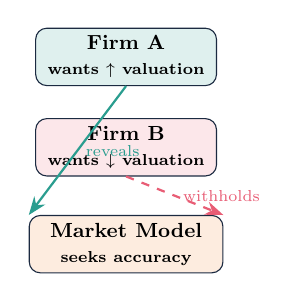
\begin{tikzpicture}[
        scale=0.82, transform shape,
        block/.style={rectangle, draw=primaryDark, fill=primaryDark!8, rounded corners=4pt, 
                      minimum width=2.8cm, minimum height=0.75cm, align=center, font=\small\bfseries},
        arrow/.style={-Stealth, thick, primaryDark}
      ]
        \node[block, fill=successGreen!15] (f1) at (0, 2.8) {Firm A\\{\scriptsize wants $\uparrow$ valuation}};
        \node[block, fill=accentCoral!15] (f2) at (0, 1.4) {Firm B\\{\scriptsize wants $\downarrow$ valuation}};
        \node[block, fill=accentGold!20, minimum width=3cm] (market) at (0, -0.1) {Market Model\\{\scriptsize seeks accuracy}};
        \draw[arrow, successGreen] (f1.south) -- node[right, font=\scriptsize, text=successGreen] {reveals} (market.north west);
        \draw[arrow, accentCoral, dashed] (f2.south) -- node[right, font=\scriptsize, text=accentCoral] {withholds} (market.north east);
      \end{tikzpicture}
    \end{column}
  \end{columns}
\end{frame}

% ======================= SLIDE 3: GAME MODEL =======================
\begin{frame}{Game-Theoretic Model}
  \begin{center}
  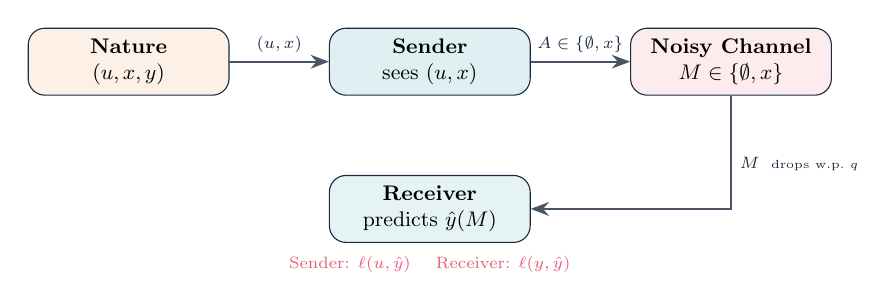
\begin{tikzpicture}[
    scale=0.85, transform shape,
    stage/.style={rectangle, draw=primaryDark, fill=primaryDark!6, rounded corners=6pt,
                  minimum width=3cm, minimum height=1cm, align=center, font=\small},
    arrow/.style={-Stealth, thick, primaryDark!80},
    label/.style={font=\scriptsize, primaryDark}
  ]
    \node[stage, fill=accentGold!15] (nature) at (0,0) {\textbf{Nature}\\$(u, x, y)$};
    \node[stage, fill=primaryTeal!12] (sender) at (4.5,0) {\textbf{Sender}\\sees $(u, x)$};
    \node[stage, fill=accentCoral!12] (channel) at (9, 0) {\textbf{Noisy Channel}\\$M \in \{\emptyset, x\}$};
    \node[stage, fill=successGreen!12] (receiver) at (4.5, -2.2) {\textbf{Receiver}\\predicts $\hat{y}(M)$};
    \draw[arrow] (nature) -- node[above, label] {$(u,x)$} (sender);
    \draw[arrow] (sender) -- node[above, label] {$A \in \{\emptyset, x\}$} (channel);
    \draw[arrow] (channel) |- node[right, label, pos=0.3] {$M$\; {\tiny drops w.p.\ $q$}} (receiver);
    \node[below=2pt of receiver, font=\scriptsize, text=accentCoral] {Sender: $\ell(u, \hat{y})$ \quad Receiver: $\ell(y, \hat{y})$};
  \end{tikzpicture}
  \end{center}
  \vspace{2pt}
  \textbf{Stackelberg game:} Receiver commits $\hat{y}$ $\to$ Sender best-responds $\to$ outcome realized.
  \vspace{4pt}
  \begin{columns}[T]
    \begin{column}{0.48\textwidth}
      \begin{alertblock}{Strategic Risk (Voluntary)}
        \vspace{-8pt}
        $$R_S := \min_{\hat{y}} \E[\ell(Y, \hat{y}(M))]$$
        \vspace{-12pt}
      \end{alertblock}
    \end{column}
    \begin{column}{0.48\textwidth}
      \begin{block}{Vanilla Risk (Mandatory)}
        \vspace{-8pt}
        $$R_V := \E[\ell(Y, \hat{y}_V(M))] \quad (A \equiv x)$$
        \vspace{-12pt}
      \end{block}
    \end{column}
  \end{columns}
  \vspace{4pt}
  \centering{\small\textbf{Strategic Advantage:} $R_S < R_V$ \quad\textemdash\quad voluntary \textit{outperforms} mandatory}
\end{frame}

% ======================= SLIDE 4: REGRESSION RESULTS =======================
\begin{frame}{Regression: Sufficiency \& Necessity}
  {\small Loss: $(y - \hat{y})^2$ (MSE).\; Linear receiver: $\hat{y}(\emptyset) = 0,\; \hat{y}(x) = b^\top x$.\; Key fields: $F(x,u) = (2u - b^\top x)\,b^\top x$,\; $G(x,y) = (2y - b^\top x)\,b^\top x$.}

  \vspace{4pt}
  \begin{alertblock}{Theorem (Sufficiency)}
    Strategic advantage exists if $\exists\, b$ such that:
    \vspace{-4pt}
    $$\|U{-}Y\|_2 \;<\; \frac{\E[|G|] - \Var(b_Y^\top X) - \Var((b{-}b_Y)^\top X)}{4\sqrt{\Var(b_Y^\top X)}}$$
    \vspace{-8pt}
  \end{alertblock}
  \vspace{-2pt}
  \begin{block}{Theorem (Necessity)}
    \vspace{-6pt}
    $$\max_b \Big(\E[|G|] - \Var(b_Y^\top X) - \Var((b{-}b_Y)^\top X)\Big) > 0$$
    \vspace{-8pt}
  \end{block}
  \vspace{4pt}
  \begin{columns}[T]
    \begin{column}{0.54\textwidth}
      {\small\textbf{Interpretation:}
      \begin{itemize}
        \item \textbf{LHS} = preference misalignment $\|U - Y\|_2$
        \item \textbf{RHS} = feature informativeness vs.\ sub-optimality
      \end{itemize}}
    \end{column}
    \begin{column}{0.44\textwidth}
      \begin{exampleblock}{}
        {\small Both conditions are \textbf{independent of $q$}!\\ $q$ scales magnitude, not existence.}
      \end{exampleblock}
    \end{column}
  \end{columns}
\end{frame}

% ======================= SLIDE 5: GAUSSIAN =======================
\begin{frame}{Gaussian Specialization}
  When $(U, X, Y) \sim \mathcal{N}(0, \Sigma)$, the sufficiency condition has a \textbf{closed-form}:

  \vspace{4pt}
  \begin{alertblock}{Theorem (Gaussian Sufficiency)}
    With $b = 2\Sigma_{XX}^{-1}\Sigma_{XU}$, strategic advantage exists if:
    $$2\bigl(b_Y^\top \Sigma_{XU} - \sigma_Z^2\bigr) + \frac{8\kappa\,\sigma_Z}{s\sqrt{2\pi}}\, e^{-\alpha^2/2} \;>\; \Sigma_{XY}^\top \Sigma_{XX}^{-1} \Sigma_{XY}$$
  \end{alertblock}
  \vspace{2pt}
  \begin{columns}[T]
    \begin{column}{0.48\textwidth}
      \begin{block}{Parameters}
        \begin{itemize}
          \item $b_Y = \Sigma_{XX}^{-1}\Sigma_{XY}$,\; $b_U = \Sigma_{XX}^{-1}\Sigma_{XU}$
          \item $\sigma_Z^2 = \Sigma_{XU}^\top \Sigma_{XX}^{-1}\Sigma_{XU}$
          \item $\kappa = \Cov(U, Y \mid X)$,\; $s^2 = \Var(U \mid X)$
        \end{itemize}
      \end{block}
    \end{column}
    \begin{column}{0.48\textwidth}
      \begin{exampleblock}{Why It Matters}
        \begin{itemize}
          \item Everything is a function of $\Sigma$
          \item Directly \textbf{verifiable} from data
          \item Provides \textbf{intuitive} parameter interpretations
        \end{itemize}
      \end{exampleblock}
    \end{column}
  \end{columns}
\end{frame}

% ======================= SLIDE 6: REGRESSION FIGURE =======================
\begin{frame}{Regression: Numerical Validation}
  \begin{columns}[c]
    \begin{column}{0.50\textwidth}
      \centering
      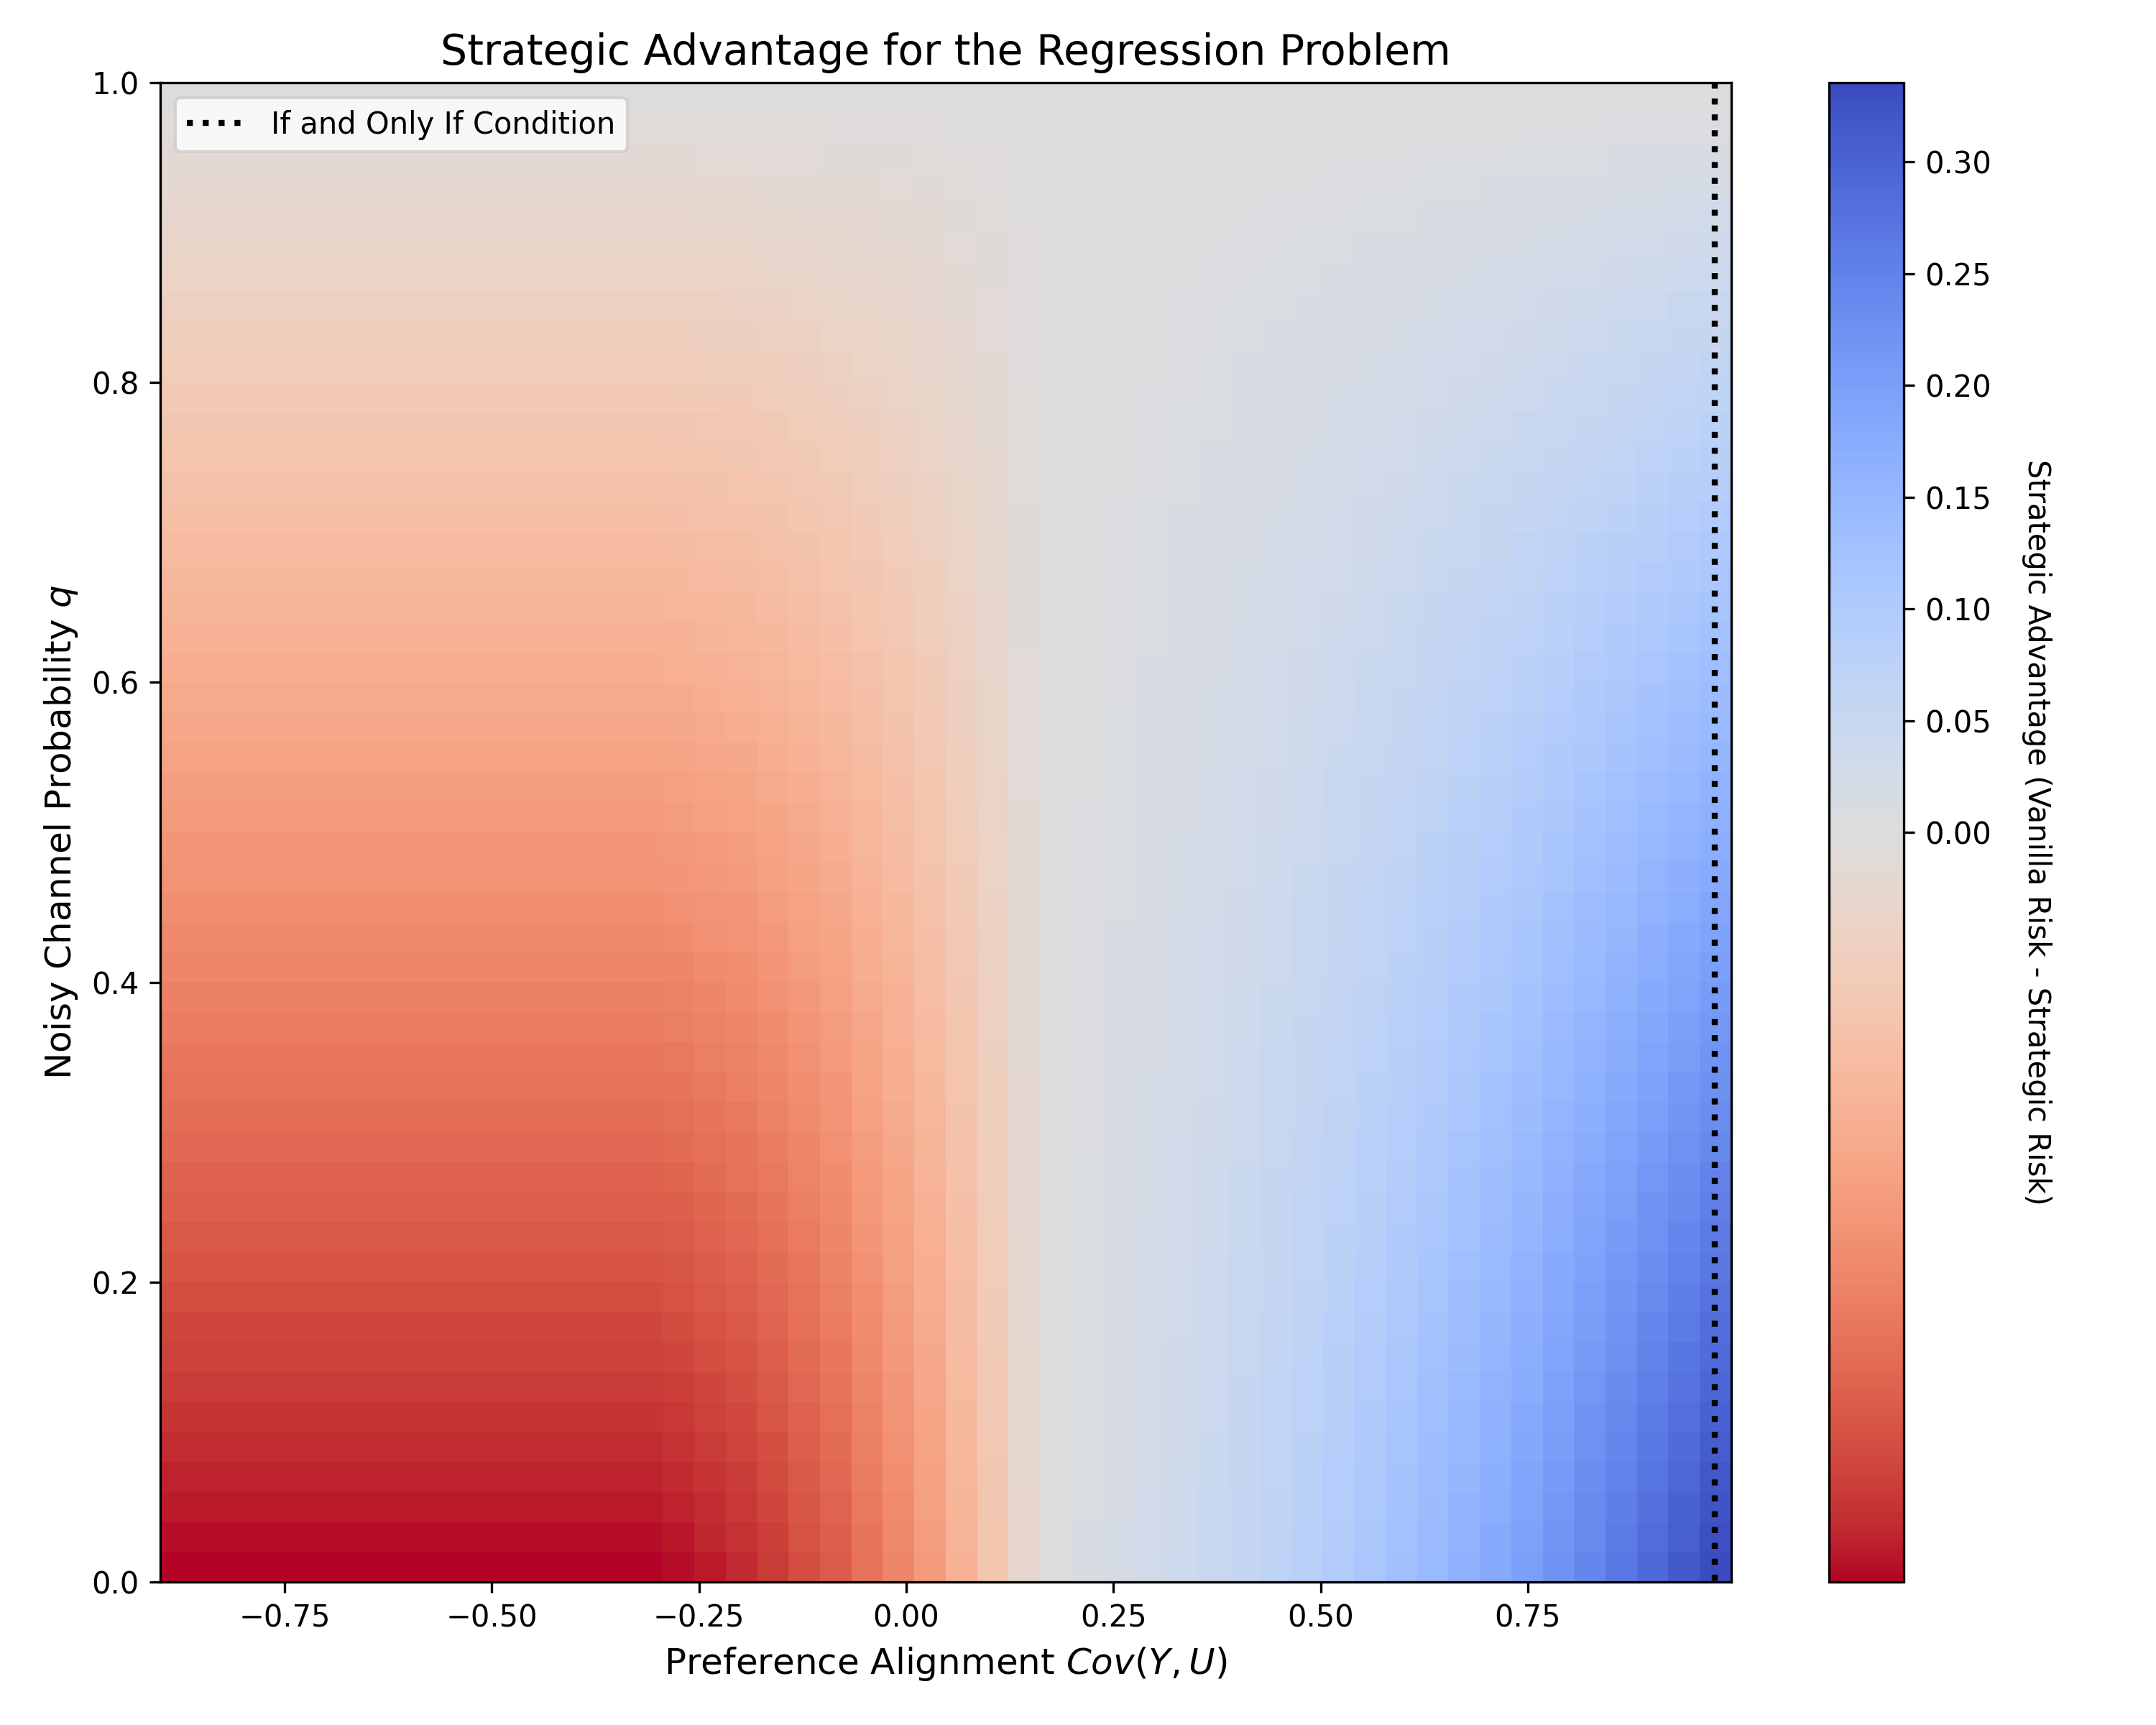
\includegraphics[width=\linewidth]{figures/regression_strategic_advantage.png}
    \end{column}
    \begin{column}{0.47\textwidth}
      \textbf{Setup:} $(X, Y, U) \sim \mathcal{N}(0, \Sigma)$
      \begin{itemize}
        \item Unit marginal variances
        \item $\Cov(X,Y) = \Cov(X,U) = 0.2$
        \item Sweep $q \in [0,1]$ and $\Cov(Y,U) \in [-1,1]$
      \end{itemize}
      \vspace{8pt}
      \begin{exampleblock}{Result}
        The analytical sufficiency bound (\textbf{dotted contour}) reliably delineates the true advantage region.\\[4pt]
        {\small Advantage region is \textbf{vertical} $\Rightarrow$ confirms independence from $q$.}
      \end{exampleblock}
    \end{column}
  \end{columns}
\end{frame}

% ======================= SLIDE 7: CLASSIFICATION =======================
\begin{frame}{Classification: Stackelberg Equilibrium}
  {\small $\cY = \{-1,+1\}$,\; $0$-$1$ loss.\; Only two strategies: default to $+1$ ($\cS_1$) or $-1$ ($\cS_{-1}$).\; Assume $\E[Y] > 0$.}
  \vspace{2pt}
  \begin{columns}[T]
    \begin{column}{0.48\textwidth}
      \begin{exampleblock}{\centering Case 1: $\cS_1$ dominates $\forall q$}
        {\small When $R_{\cS_1}^\star(0) \le R_{\cS_{-1}}^\star(0)$:}
        \vspace{-6pt}
        \begin{align*}
          &(1{-}q)\biggl[\E\!\left[\tfrac{1-|\eta|}{2}\right] - \pi_{-1}\E\!\left[\tfrac{1-|\eta_{-1}|}{2}\right]\\
          &\quad - \pi_1\Prob(Y\!=\!{-1} \mid U\!=\!1)\biggr] > 0
        \end{align*}
        \vspace{-10pt}
        
        {\scriptsize \textcolor{successGreen}{\textbf{Independent of $q$}} (like regression)}
      \end{exampleblock}
    \end{column}
    \begin{column}{0.48\textwidth}
      \begin{alertblock}{\centering Case 2: Switch at $q^\star$}
        {\small $\exists\, q^\star$: use $\cS_1$ for $q \ge q^\star$, $\cS_{-1}$ for $q < q^\star$:}
        \vspace{-6pt}
        \begin{align*}
          &(1{-}q)\!\left[\E\!\left[\tfrac{1-|\eta|}{2}\right] - \pi_1\E\!\left[\tfrac{1-|\eta_1|}{2}\right]\right]\\
          &+ q\left[\Prob(Y\!=\!{-1}) - \pi_1\Prob(Y\!=\!1 \mid U\!=\!1)\right]\\
          &> \pi_{-1}\Prob(Y\!=\!1 \mid U\!=\!{-1})
        \end{align*}
        \vspace{-10pt}
        
        {\scriptsize \textcolor{accentCoral}{\textbf{Depends on $q$}} (unlike regression)}
      \end{alertblock}
    \end{column}
  \end{columns}
  \vspace{4pt}
  \begin{center}
    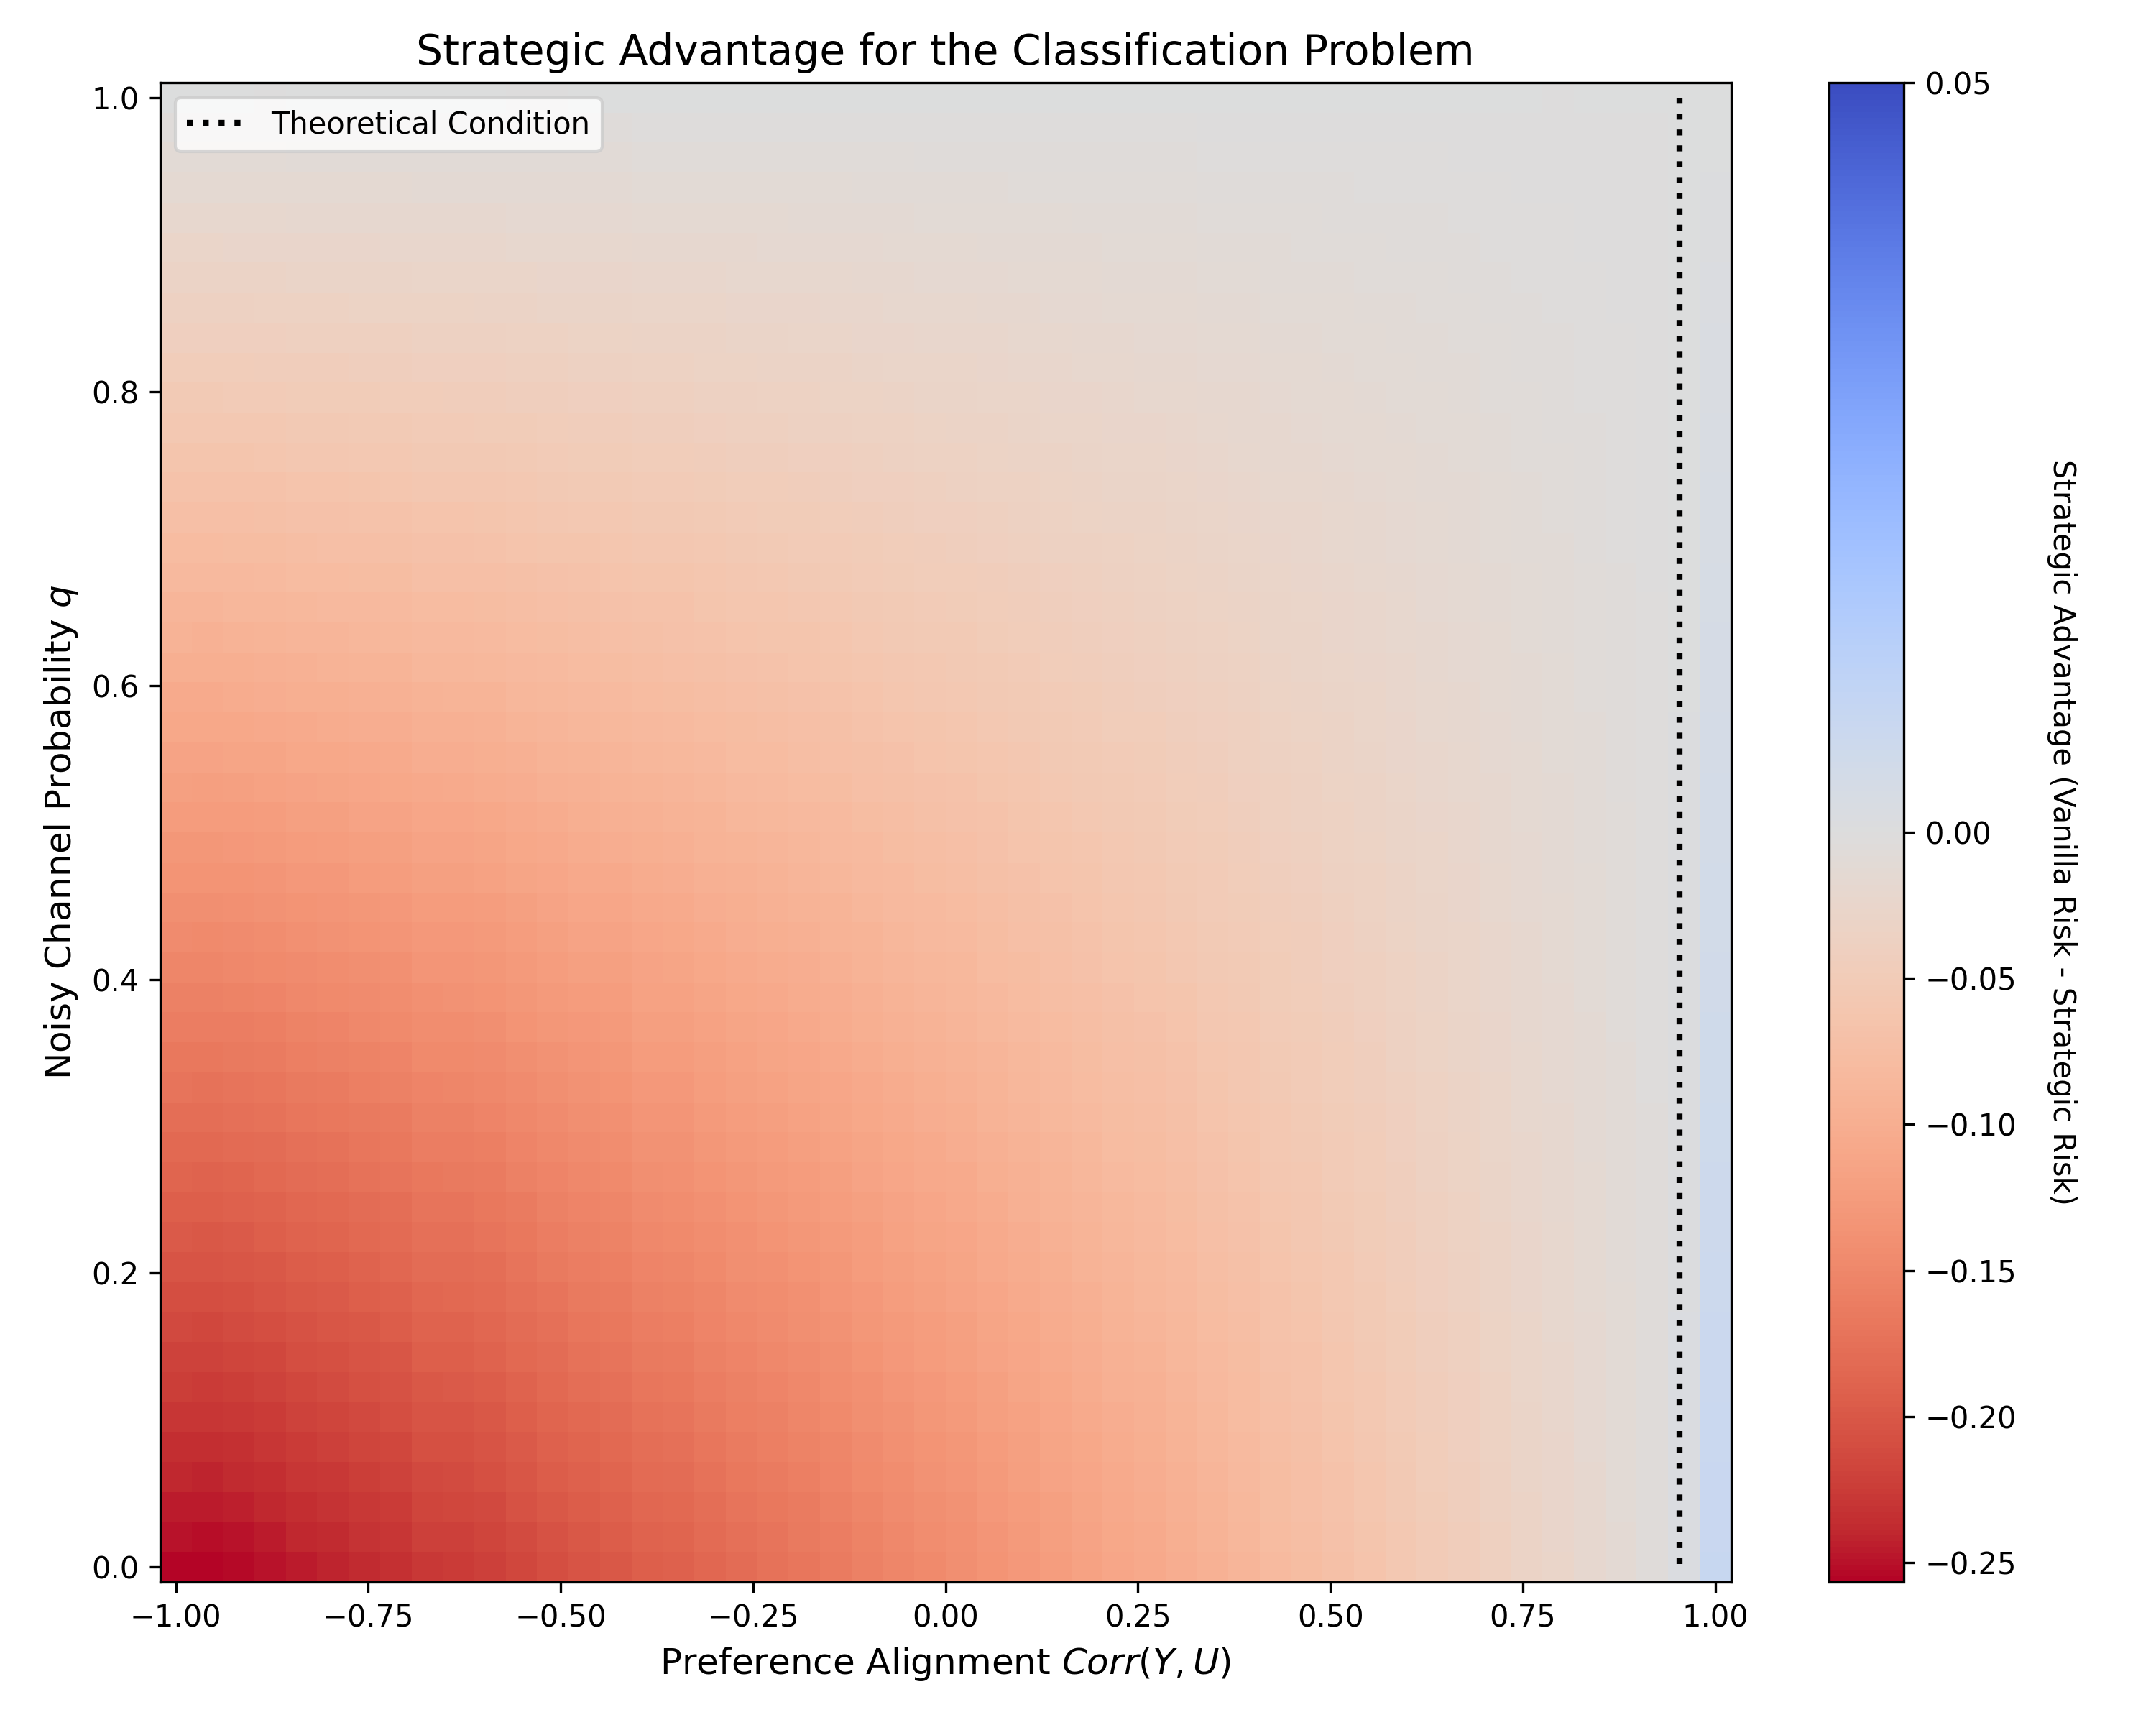
\includegraphics[width=0.38\linewidth]{figures/classification_strategic_advantage.png}
  \end{center}
\end{frame}

% ======================= SLIDE 8: ONLINE LEARNING =======================
\begin{frame}{Online Learning: Unknown Environment}
  \begin{alertblock}{Challenge}
    Previous results assume known distributions. Now the receiver must \textbf{learn} through repeated interaction.
  \end{alertblock}
  \vspace{2pt}
  \begin{columns}[T]
    \begin{column}{0.52\textwidth}
      \textbf{Bayesian Adaptive Protocol:}
      \begin{enumerate}
        \item Initialize prior $p_1(\theta)$ over $\Theta$
        \item Each round $t$: select regime $D_t$, commit $\hat{y}_t$, observe $y_t$
        \item Update: $p_{t+1}(\theta) \propto p_t(\theta) \cdot \Prob(M_t, y_t \mid \theta, \hat{y}_t)$
      \end{enumerate}
      \vspace{4pt}
      \textbf{Regret:} $\mathcal{R}_T = \sum_t \ell(y_t, \hat{y}_t(M_t)) - T \cdot \min\{R_V^\star, R_S^\star\}$
    \end{column}
    \begin{column}{0.45\textwidth}
      \begin{exampleblock}{\centering Regret Guarantee}
        \vspace{-2pt}
        $$\boxed{\E[\mathcal{R}_T] \le C\sqrt{T}}$$
        \vspace{-4pt}
        
        {\small Decomposition:}
        \begin{itemize}
          \item \textbf{Estimation:} $O(\sqrt{T})$
          \item \textbf{Regime ID:} $O(\log T)$
        \end{itemize}
        \vspace{2pt}
        {\small $\Rightarrow$ Converges to optimal regime!}
      \end{exampleblock}
    \end{column}
  \end{columns}
\end{frame}

% ======================= SLIDE 9: SUMMARY =======================
\begin{frame}{Summary \& Future Directions}
  \begin{center}
  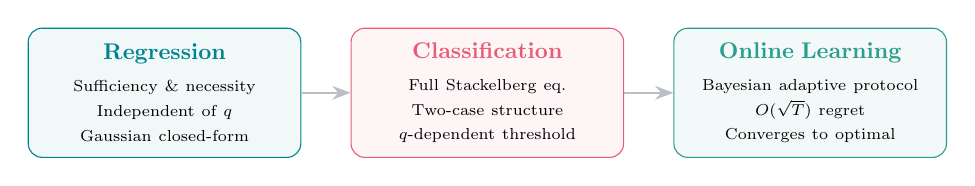
\begin{tikzpicture}[
    scale=0.82, transform shape,
    card/.style={rectangle, draw=#1, fill=#1!6, rounded corners=5pt,
                 minimum width=4cm, minimum height=2cm, align=center, 
                 text width=3.8cm, font=\small, inner sep=6pt}
  ]
    \node[card=primaryTeal] (r) at (0, 0) {
      {\normalsize\textbf{\textcolor{primaryTeal}{Regression}}}\\[3pt]
      {\scriptsize Sufficiency \& necessity}\\
      {\scriptsize Independent of $q$}\\
      {\scriptsize Gaussian closed-form}
    };
    \node[card=accentCoral] (c) at (5, 0) {
      {\normalsize\textbf{\textcolor{accentCoral}{Classification}}}\\[3pt]
      {\scriptsize Full Stackelberg eq.}\\
      {\scriptsize Two-case structure}\\
      {\scriptsize $q$-dependent threshold}
    };
    \node[card=successGreen] (o) at (10, 0) {
      {\normalsize\textbf{\textcolor{successGreen}{Online Learning}}}\\[3pt]
      {\scriptsize Bayesian adaptive protocol}\\
      {\scriptsize $O(\sqrt{T})$ regret}\\
      {\scriptsize Converges to optimal}
    };
    \draw[-Stealth, thick, primaryDark!30] (r) -- (c);
    \draw[-Stealth, thick, primaryDark!30] (c) -- (o);
  \end{tikzpicture}
  \end{center}
  \vspace{6pt}
  \begin{columns}[T]
    \begin{column}{0.48\textwidth}
      \begin{alertblock}{\centering Limitations}
        {\small
        \begin{itemize}
          \item Conservative sufficiency bounds
          \item Linear strategies only (regression)
          \item Parametric environment (online)
        \end{itemize}}
      \end{alertblock}
    \end{column}
    \begin{column}{0.48\textwidth}
      \begin{exampleblock}{\centering Future Work}
        {\small
        \begin{itemize}
          \item Non-linear predictors
          \item Multi-sender competition
          \item Partial feature disclosure
          \item Tighter bounds
        \end{itemize}}
      \end{exampleblock}
    \end{column}
  \end{columns}
\end{frame}

% ======================= SLIDE 10: THANK YOU =======================
{
\setbeamercolor{background canvas}{bg=primaryDark}
\begin{frame}[plain, noframenumbering]
  \vfill
  \begin{center}
    {\Huge\color{white}\textbf{Thank You!}}\\[14pt]
    {\Large\color{accentCoral}Questions \& Discussion}\\[20pt]
    {\color{white!60}\large Author 1\textsuperscript{1} \quad \& \quad Author 2\textsuperscript{2}}\\[14pt]
    \tikz{
      \node[draw=accentGold, fill=accentGold!12, rounded corners=6pt, inner sep=10pt, text width=0.72\textwidth, align=center] {
        \color{primaryDark}\textbf{Key Message}\\[4pt]
        \color{primaryDark}\textit{Voluntary disclosure can outperform mandatory disclosure}\\
        \color{primaryDark}\textit{when preferences are sufficiently aligned with ground truth.}
      };
    }
  \end{center}
  \vfill
\end{frame}
}

\end{document}
